\documentclass{article}

\usepackage[%
    left=0.5in,%
    right=0.5in,%
    top=0.5in,%
    bottom=0.5in,%
]{geometry}%
\usepackage{minitoc}
\usepackage{multicol}
\usepackage{graphicx}
\usepackage{fixltx2e}
\usepackage{listings}
\usepackage{color}
\usepackage{hyperref}
    \hypersetup{ colorlinks = true, linkcolor = blue }
\usepackage{blindtext}
\definecolor{lightgray}{gray}{0.9}
\graphicspath{ {./} }

\newcommand{\inlinecode}[2]{\colorbox{lightgray}{\lstinline
[language=#1]$#2$}}
\newcommand{\worddef}[1]{\hyperref[sec:reference]{\textit{#1}}}

\begin{document}

\tableofcontents

\newpage

\section{Kinds of agent architectures}
\begin{itemize}
  \item \textbf{uniform architectures}
  \begin{itemize}
    \item reactive architectures 
    \item deliberative architectures. Much more complex architectures (problem solving, search)
  \end{itemize}
  \item \textbf{hybrid architectures}: reactive and deliberative components. Often used for more complex robotic tasks 
  \item \textbf{multi-agent system architectures} – agents may have uniform or hybrid architectures (usually with additional coordination component(s))
\end{itemize}

\section{Simple reactive architectures}

\begin{flushleft}
Actions are directly triggered by percepts.
\begin{itemize}
  \item no representations of the environment, meaning no goals
  \item predefined, fixed response to a situation. Always have the same response to a same situation
  \item fast response to changes in the environment
\end{itemize}
\end{flushleft}

\section{Action selection function}

\begin{itemize}
  \item the action selection function for a simple reactive agent looks like $selectAction : Event \rightarrow Action$
  \item i.e., it responds only to single events in a predetermined way 
  \item add state to respond to sequences of events (next lecture)
\end{itemize}

\section{What's in a percept?}

\begin{itemize}
  \item Russell and Norvig model action selection as a function that takes a \textbf{single input} (percept) to a \textbf{single unique output} (action) 
  \item this is fine if we allow percepts and actions to be arbitrarily complex 
  \item e.g., if the output of all the agent’s sensors are combined into a single percept on the basis of which the agent chooses a single composite action
  \item Because an agent can have multiple sensors, it becomes inefficient to use a look-up table as the amount of input value combinations grow exponentially.
  \item however it is more natural to view the \textbf{output of each of the agent’s sensors as a distinct percept}, and each of the atomic actions the agent can perform as different actions 
  \item gives a more compact representation of the task environment (we don’t have to enumerate all possible combinations of sensor outputs and effector inputs
  \item however action selection becomes more complex
  \item need to be able to combine the outputs of a \textit{set of action selection functions}
\end{itemize}

\section{Action selection}
\begin{itemize}
  \item same percept may trigger multiple actions 
  \item actions can be combined in various ways:
  \begin{itemize}
    \item multiple actions may be executed in \textbf{parallel}
    \item one action may take \textbf{precedence} over the others
    \item combined into a \textbf{single action}
  \end{itemize}
\end{itemize}

\begin{multicols}{2}

\subsection{Parallel actions}

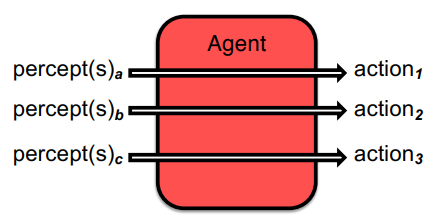
\includegraphics[scale=0.5]{paralel_actions.png}

\subsection{Prioritised actions}

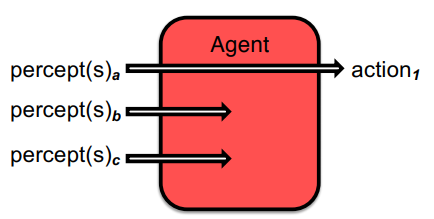
\includegraphics[scale=0.5]{prioritised_actions.png}

\subsection{Combined actions}

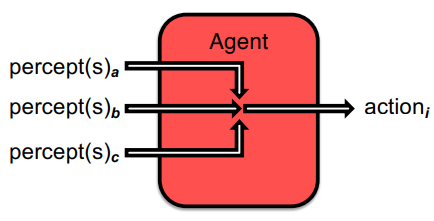
\includegraphics[scale=0.5]{combined_actions.png}

\end{multicols}

\section{Boids}
\begin{itemize}
  \item a boid is a simple agent that navigates according to its local perception of its environment, the simulated physics of the environment and a set of simple behavioural rules:
  \begin{itemize}
     \item collision avoidance: avoid collisions with nearby boids (and static obstacles)
     \item velocity matching: attempt to match velocity with nearby boids 
     \item flock centring: attempt to stay close to nearby boids
   \end{itemize} 
  \item each boid also has a ‘migratory urge’, a global direction or position towards which the boids will fly
\end{itemize}

\section{Advantages of simple reactive architectures}
\begin{itemize}
  \item simple architectures can produce complex behaviour 
  \item no representations of the environment or complex problem solving required 
  \item can use dedicated, parallel hardware 
  \item fast (often real-time) response to changes in the environment
\end{itemize}

\section{Disadvantages of simple reactive architectures}
\begin{itemize}
  \item fixed response to a given situation 
  \item all responses must be defined in advance 
  \item can’t cope with novel situations for which they don’t have a predefined behaviour 
  \item can’t solve some problems at all
\end{itemize}


\pagebreak
\section*{Reference section} \label{sec:reference}
\begin{description}
	\item[placeholder] \hfill \\
\end{description}
\end{document}
